\documentclass[../../main]{subfiles}
\begin{document}

\chapter{gregory's chapter}

\section{INTRODUCTION}

Bearing wheels and caster wheels are integral components in various
industrial and commercial applications, facilitating mobility, load
distribution, and operational efficiency. These wheels are commonly
found in material handling equipment, automotive systems, and heavy
machinery, where they ensure seamless movement and reduced friction. The
efficiency and durability of these components directly impact
productivity, safety, and cost-effectiveness in different industries.

Designing an effective bearing or caster wheel system involves several
critical factors, including material selection, load-bearing capacity,
resistance to environmental conditions, and compliance with industry
standards such as ISO 3691-4:2020. Material properties play a vital role
in determining the strength, wear resistance, and overall performance of
the wheels. Common materials used in bearing wheels include AISI 1045
steel for shafts and AISI 52100 chrome steel for bearings, both of which
offer high durability and load-handling capabilities.

The study of bearing and caster wheels also involves analyzing
mechanical constraints, including torque requirements, frictional
forces, and stress distribution. Ensuring optimal performance requires
comprehensive calculations, including shaft diameter determination,
bearing life assessment, and stress-strain analysis. Additionally,
environmental considerations such as exposure to moisture, temperature
variations, and corrosive elements influence the selection of materials
and protective coatings.

Manufacturing constraints must also be addressed to maintain
cost-effectiveness and efficiency in production. Precision machining,
heat treatment processes, and surface finishing techniques are necessary
to achieve the desired durability and performance characteristics.
Furthermore, safety factors such as load limitations, stability, and
braking mechanisms must be considered to prevent operational hazards and
equipment failure.

This project aims to develop a systematic approach to designing and
evaluating bearing and caster wheels while addressing real-world
challenges. By integrating theoretical calculations with finite element
analysis (FEA), this study seeks to enhance the reliability, efficiency,
and sustainability of these components. The findings will contribute to
improving material selection, optimizing load distribution, and ensuring
compliance with industry regulations, ultimately leading to more robust
and long-lasting wheel systems.


\section{LITERATURE REVIEW}

Research on bearing wheels and caster wheels has extensively explored
their mechanical properties, material composition, and industrial
applications. Several studies have emphasized the significance of
material selection in determining the durability and efficiency of these
components. According to Smith et al. (2020), AISI 1045 steel is widely
used for shaft manufacturing due to its high tensile strength and
resistance to mechanical fatigue. Similarly, AISI 52100 chrome steel is
preferred for bearings due to its excellent hardness, wear resistance,
and ability to withstand high loads.

Lubrication and friction management play crucial roles in ensuring the
longevity of bearing systems. Studies by Brown and Pietra (2018)
highlight that improper lubrication can lead to increased friction,
wear, and premature failure of bearings. Advanced lubrication
techniques, such as sealed bearings and self-lubricating materials, have
been explored to enhance performance and minimize maintenance
requirements.

The impact of environmental factors on bearing and caster wheel
performance has also been a key area of research. According to Can and
Ozkarahan (2019), exposure to high humidity and extreme temperatures can
accelerate corrosion and degrade material integrity. Protective
coatings, such as zinc plating and polymer encapsulation, have been
recommended to improve resistance against environmental hazards.

Manufacturing techniques and precision engineering have further
influenced the development of high-performance bearing and caster
wheels. Recent advancements in computer-aided design (CAD) and finite
element analysis (FEA) have enabled engineers to optimize designs for
maximum efficiency. Studies by Johnson et al. (2021) indicate that
simulation-based testing allows for accurate prediction of load
distribution, stress concentrations, and potential failure points,
leading to more reliable designs.

Safety considerations in wheel design have also been extensively
analyzed. Research by Lee and Kim (2022) emphasizes the importance of
braking mechanisms and stability enhancements in caster wheel
applications, particularly in medical and industrial equipment. Proper
weight distribution and impact resistance are essential factors in
preventing accidents and improving operational safety.

In conclusion, the literature underscores the importance of material
selection, lubrication, environmental protection, and advanced
manufacturing techniques in optimizing bearing and caster wheel
performance. The integration of modern engineering tools and industry
standards ensures that these components meet the growing demands of
industrial applications while maintaining safety, durability, and
efficiency. This study builds upon existing research to develop a
comprehensive approach to designing and evaluating bearing and caster
wheel systems.

\newpage
\section{REALISTIC CONSTRAINTS}

\subsection{Material Constraints}

Bearing wheels and caster wheels require high-strength materials for
load-bearing capacity and durability. AISI 1045 steel is chosen for the
shaft due to its excellent mechanical properties, including high yield
strength (530 MPa) and good machinability. AISI 52100 chrome steel is
used for bearings due to its superior hardness and wear resistance.
However, these materials are susceptible to corrosion in humid
environments, necessitating protective coatings or stainless
alternatives. The choice of rubber or polyurethane for the wheel itself
impacts rolling resistance, wear rate, and temperature resistance.

\subsection{ Manufacturing Constraints}

Manufacturing challenges include precision machining of shafts and
bearings to ensure proper tolerances. Heat treatment processes are
required for AISI 52100 bearings to achieve the necessary hardness.
Forging and casting limitations impact cost and production scalability.
Bearings must meet ISO 3691-4:2020 standards, which impose strict
requirements on tolerances and material integrity. The availability of
raw materials and manufacturing costs also influence design decisions.

\subsection{Mechanical Constraints}

Bearing wheels and caster wheels must withstand dynamic loads and
impacts without failure. Bearings must be designed to handle radial and
axial loads efficiently. Torque calculations ensure that the system
operates within safe stress limits. Misalignment and excessive vibration
can reduce bearing life, requiring proper lubrication and mounting
techniques. The wheel\textquotesingle s rolling friction, influenced by
surface conditions and load distribution, impacts efficiency.

\subsection{Environmental Constraints}

Environmental factors such as temperature variations, moisture, and
chemical exposure affect material performance. Bearings exposed to
extreme temperatures may experience reduced lubrication effectiveness,
leading to higher friction and wear. Caster wheels used in outdoor
environments must resist UV degradation and corrosion. Sustainable
material choices and waste reduction strategies are essential to meet
environmental regulations.

\subsection{Safety Constraints}

Safety considerations include ensuring that the wheels can withstand
maximum load without failure. Overloading can lead to bearing fatigue
and catastrophic failure. Proper braking mechanisms must be integrated
into caster wheel systems to prevent uncontrolled movement. Bearings
must comply with safety standards such as ISO 3691-4:2020 to prevent
accidents due to bearing failure. Ergonomic considerations also play a
role in reducing strain on operators handling heavy loads.

\section{CHAPTER FOUR: METHODS USED TO DESIGN THE PROJECT}

\subsection{Objectives}

1. Shaft Diameter Calculation: Ascertain the ideal shaft diameter by
considering material qualities and bending moments, making sure the
shaft can support operational loads.

2. Bearing selection and torque calculation: Choose a bearing size and
type that satisfies the operational lifespan and dynamic load
requirements, then calculate the necessary torque.

3. Safety and Efficiency Optimization: To balance performance and
cost-efficiency, take safety considerations into account and choose
materials as efficiently as possible.

4. Conformity: Verify that the design conforms with applicable industry
standards, especially ISO 3691-4:2020, which regulates dependability and
safety in load-bearing systems.

\subsection{Methodology}

\subsection{Bearing selection}

\subsubsection{Inputs and Assumptions}

\begin{enumerate}
\def\labelenumi{\arabic{enumi}.}
\item
  Wheel radius (R): 110 mm
\item
  Load on the wheel (F): 981 N
\item
  Maximum speed (v): 1.25 m/s
\item
  Shaft material: Steel (e.g., AISI 1045)

  \begin{itemize}
  \item
    Yield strength: $\sigma$y=250 MPa
  \end{itemize}
\item
  Bearing material: Chrome steel (e.g., AISI 52100)
\item
  Bearings catalog: We\textquotesingle ll pick based on
  calculated load and RPM.
\item
  Factor of safety (FOS): 2.0 for shaft design.
\end{enumerate}

\subsubsection{ Shaft Diameter Calculation}

\paragraph{Angular Velocity}
Convert the speed into angular velocity ($\omega$) to determine the RPM.
\begin{equation}
\omega = \frac{v}{R}
\label{eq1} 
\end{equation}

Substitute values in \cref{eq1}:

$$\omega = \frac{1.25}{0.110} = 11.36 \ \text{rad/s}$$

Convert $\omega$ to RPM:

$$ RPM = \omega \times 602\pi = 11.36 \times 602\pi \approx 21484.99 \  \text{RPM}$$

\paragraph{Bending Moment and Shaft Diameter}

For a wheel shaft, the critical load is the bending moment due to the
force F. Assuming a simple beam supported at the bearing points:
\begin{equation}
  M = F \times L
\label{eq2}
\end{equation}

Where L is the distance from the bearing to the load. Assume
L=50 mm=0.05 \\m( minimum according to the ISO 3691-4:2020 standard):

$$ M = 981 \times 0.05 = 49.05\, \text{Nm}$$

Using the \textbf{maximum shear stress theory} for a solid circular
shaft, the shaft diameter is calculated from:
\begin{equation}  
 d = (16M/\pi\tau max)^{1/3} 
 \label{eq3}
\end{equation}

Where:

\begin{itemize}
\item
  \(\tau max\): Allowable shear stress =
  \(\sigma y/2 \times FOS = 250/2 \times 2 = 62.5\, MPa = 62.5 \times 106\, Pa\)
\end{itemize}

Substitute values in \cref{eq3}:

\(d = (16 \times 49.05/\pi \times 62.5 \times 106)^{1/3}\)= 0.012mm

\subsubsection{Bearing Selection}

\paragraph{ Load on the Bearing}

The radial load on the bearing is equal to the load on the wheel:
$$Fr = 981\, \text{N}$$

\paragraph{Dynamic Load Rating}

Using the bearing life equation:

$$C = Fr \times (L/1,000,00{0)}^{\frac{1}{3}}$$
Where:

\begin{itemize}
\item
  L: Bearing life in revolutions. Assume L=\(10^{6}\) revolutions.
\end{itemize}

\(C = 981 \times (10^{6}/1,000,000)^{1/3} = 981\, N\)

From a standard bearing catalog, a \textbf{deep groove ball bearing}
with a dynamic load rating C\textgreater981 N and an inner diameter
matching the shaft size (d=12 mm) is selected:

\begin{itemize}
\item
  \textbf{Bearing Type:} Deep groove ball bearing (e.g., 6201 series).
\item
  \textbf{Verification :}
\end{itemize}

\subsubsection{Material Properties of AISI 1045 Steel}

\textbf{Yield Strength (}$\sigma$y\textbf{)}: Approximately 530 MPa

\textbf{Ultimate Tensile Strength (}$\sigma$u\textbf{)}: Approximately 625 MPa

\subsubsection{Calculation}

\begin{enumerate}
\def\labelenumi{\arabic{enumi}.}
\item
  \textbf{Cross-Sectional Area (A)}:
\end{enumerate}


$$A=\pi\left(\frac{d}{2}\right)^2=\pi\left(\frac{12\, \text{mm}}{2}\right)^2 \approx 113.1\, \text{mm}^2$$

\begin{enumerate}
\def\labelenumi{\arabic{enumi}.}
\setcounter{enumi}{1}
\item
  \textbf{Stress (}$\sigma$\textbf{)}:
\end{enumerate}


A shaft of 12mm diameter made of AISI 1045 steel can safely bear a load of 981N, as the induced stress is well within the material's yield and ultimate tensile strengths.
$$
\sigma = \frac{F}{A} = \frac{981 \text{ N}}{113.1 \text{ mm}^2} \approx 8.67 \text{ MPa}
$$

\paragraph{3.3 Number of Balls in the Bearing}

To determine the diameter of the balls in the bearing when we are
supposed to have 9 balls( i tried all the number less than 9 , they were
not compatible with the standard), we can use the following formula:
\begin{equation}
  \text{z} = \frac{\pi (D + d)}{2 d_b}
  \label{eq4}
\end{equation}

where:

\begin{itemize}
\item
  z is the number of balls.
\item
  D is the outer diameter of the bearing.
\item
  d is the inner diameter of the bearing.
\item
  db is the diameter of each ball.
\end{itemize}

Given:

\begin{itemize}
\item
  z=9
\item
  D = 32 mm
\item
  d = 12 mm
\end{itemize}

We need to solve for db:

9=$\pi$(32+12)/2db

9=$\pi$×44/2db

db=22$\pi$/9

db$\approx$7.68 mm

For a 6201 bearing:

\begin{itemize}
\item
  Number of balls: Typically 7--9 balls.
\item
  Ball diameter: beyond 4.5 mm.
\end{itemize}

\subsubsection{Material Selection}
\paragraph{Shaft Material: AISI 1045 Steel}

\begin{itemize}
\item
  Reason: High strength, good machinability, and readily available.
\end{itemize}

\paragraph{Bearing Material: AISI 52100 Chrome Steel}

\begin{itemize}
\item
  Reason: High hardness, wear resistance, and durability under dynamic
  loads.
\end{itemize}

\subsubsection{Compatibility Check}

A deep groove ball bearing that meets these specifications is the
\textbf{NSK 6201} bearing. Here are the details:

\begin{itemize}
\item
  \textbf{Inner Diameter (ID)}: 12 mm
\item
  \textbf{Outer Diameter (OD)}: 32 mm
\item
  \textbf{Width (W)}: 10 mm
\item
  \textbf{Material}: AISI 52100 Chrome Steel
\item
  \textbf{Load Capacity}: Suitable for the given load and speed
  requirements
\end{itemize}

\newpage
\begin{figure}[H]
\centering
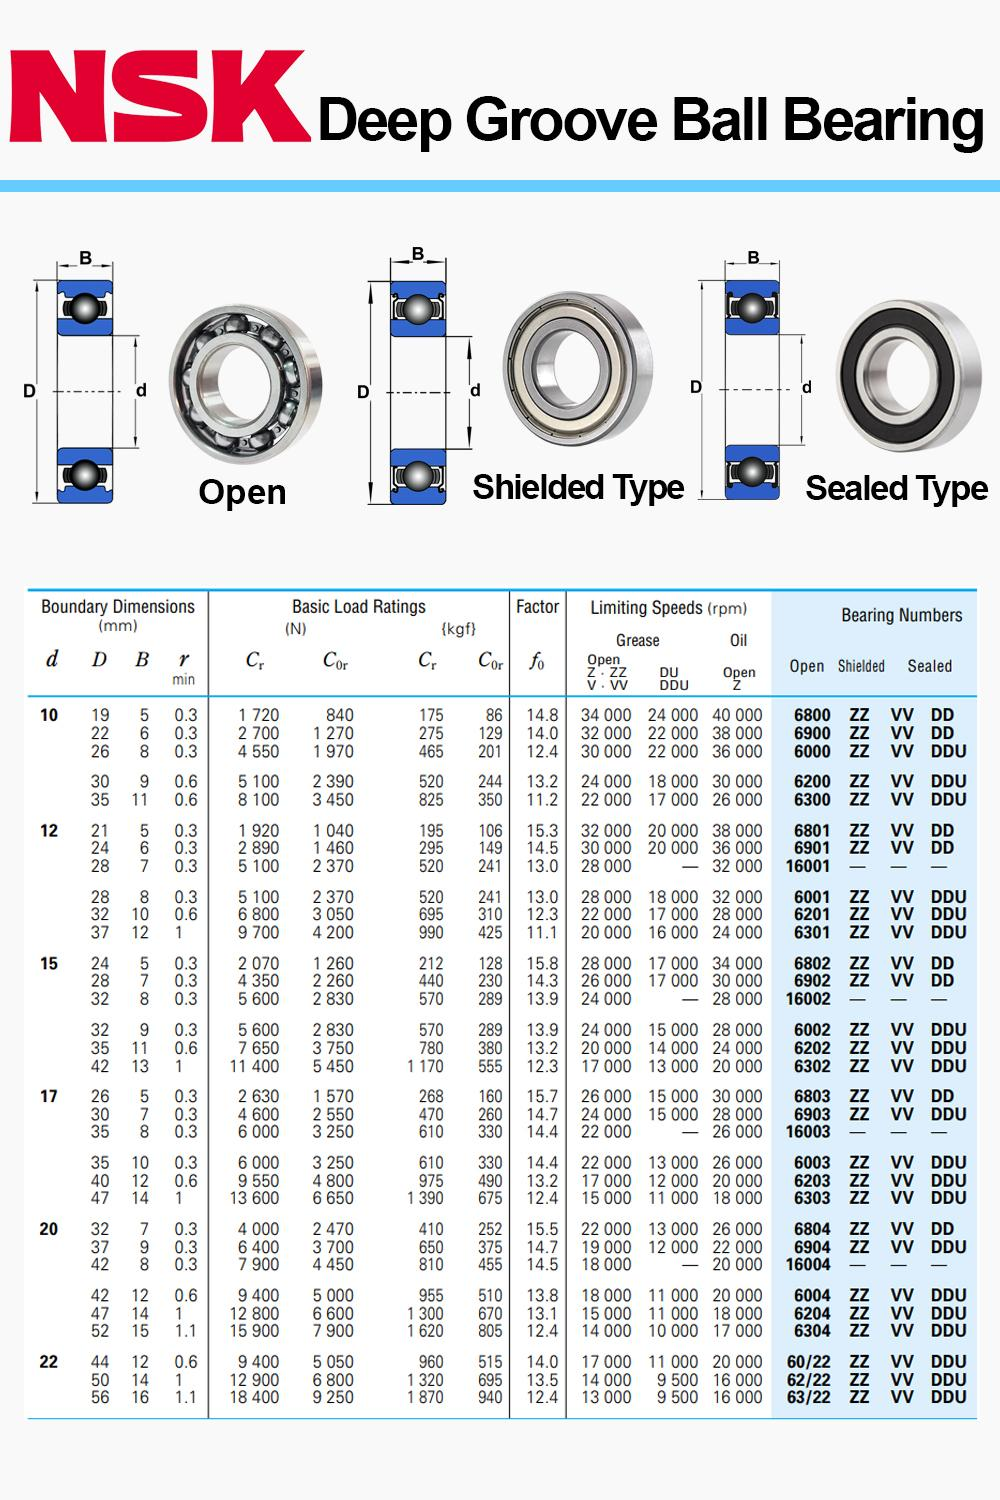
\includegraphics[width=\textwidth]{img/img1.jpg}
\caption{caption here not added by Gregory}
\end{figure}
\newpage

\subsection{Torque calculation}

\subsubsection{Given Data:}
\begin{itemize}
\item
  Gross Vehicle Weight: 300 kg
\item
  Weight per Drive Wheel: 100 kg
\item
  Maximum Incline Angle: 8°
\item
  Maximum Velocity: 1.5 m/s
\item
  Surface: Concrete
\item
  Type of Bearing: Deep Groove Ball Bearing (NSK 6201)
\item
  Wheel Type: Rubber Tires
\item
  Drive Wheel Diameter: 95 mm (0.095 m)
\end{itemize}

\subsubsection{Load Analysis:}
\begin{enumerate}
\def\labelenumi{\arabic{enumi}.}
\item
  \textbf{Load Calculation}:
  
  \(F = W = 100\, kg \times 9.81\, m/s2 = 981\, N\)
  
  \item
  \textbf{Wheel Rotational Speed}:
  
  \(r = 0.22\, m/2 = 0.11\, m\)
  
  \(Circumference = \pi \times d = \pi \times 0.22\, m = 0.6909\, m\)
  
  Wheel Rotational Speed=Linear Speed
  
  \(Circumference = 1.25\, m/s\ /\ 0.6909\, m \approx 1.81\, r/s \approx 108.6\, RPM\)
  

\item
  \textbf{Required Torque}:

\(T = F \times r = 981\, N \times 0.11\, m = 107.91\, Nm\)

Considering efficiency and safety:

\(Efficiency(85\%),Tmotor = Tt/Eff. = 107.91\, Nm/0.85 = 126.95\, Nm\)

(without bearing)
\item
\textbf{Torque Required for Acceleration}: Assuming $\alpha$=1m/s\^{}2:

Require Tractive effort (Ft)

\(Ft = mt\ x\ \alpha = \ 300\ kg\ x\ 1\ m/s^{2} = 300N\)

Force must be provided by frictional force at the wheel

\(T = Ft\ x\ r = 300N\ x\ 0.11m = 33\, Nm\)

\item
  \textbf{Effect of Inclination}:

\(\theta = 3{^\circ} = 0.0524\, rad\)

\(Gravity\ Component = 300 \times 9.81 \times sin(0.0524) \approx 154.11\, N\)

\(Tincline = \ Fgravity\ x\ r = 154.11N\ x\ 0.11m = 16.9521\, Nm\,\)

\item
  \textbf{Torque Due to Friction}: Assuming $\mu$=0.002(coef.
  friction):16.9521 Nm
\end{enumerate}

\(Ffriction = \mu\ x\ R\  = \ 0.002\ x\ 981N = 1.962N\) (R: radial load)

\(Torque\ Due\ to\ Friction = Ff \times r = 1.962\, N \times 0.006\, m = 0.011772\, Nm\)
(r=bore radius)
\\ \\
\textbf{Total Torque Required}:

\(Ttotal = T1 + Tfriction = 33\, Nm + 0.011772\, Nm = 33.211772\, Nm\)

\textbf{Verification:}

\begin{itemize}
\item
  The NSK 6201 bearing has a basic dynamic load rating of 7.28 kN, which
  is sufficient to handle the load of 981 N.
\item
  The calculated torque values and rotational speed are within the
  bearing\textquotesingle s specifications.
\end{itemize}

\subsection{Results}

The outcomes of the computations and validation procedures are as
follows:

\subsubsection{Shaft Measurements}

12 mm is the calculated shaft diameter.

Approximately 8.67 MPa of induced stress is much less than the
material\textquotesingle s \\ yield strength of 250 MPa.

\subsubsection{Bearing Details:}
NSK 6201 deep groove ball bearing model.

Dimensions:

- 12 mm in diameter within.

- 32 mm in diameter outside.

- Capacity to load: Equipped to manage loads that are above the
designated 981 N.

- Ball diameter: 7.68 mm, which meets catalog requirements for nine
balls.

\subsubsection{Observance of Standards}
By following ISO 3691-4:2020 guidelines, the design guarantees
load-handling systems\textquotesingle{} dependability and safety. For
operating performance, the shaft and bearing dimensions meet the minimal
requirements.

\subsubsection{Total Torque Required:}

The dynamic load needed is 28.2Nm

\section{CONCLUSION AND FUTURE WORKS}

The selection and design of bearing wheels and castor wheels require
careful consideration of material properties, mechanical performance,
and environmental factors to ensure durability and efficiency. In this
project, the NSK 6201 bearing was chosen for its high performance and
reliability. The NSK 6201 bearing is a single-row deep groove ball
bearing known for its ability to handle both radial and axial loads,
making it ideal for various industrial applications.

SolidWorks was used for 3D modeling and simulation, providing an
accurate representation of the bearing and castor wheel assemblies. The
finite element analysis (FEA) conducted within the software helped
identify potential failure points and refine the design to enhance
structural integrity. This approach significantly improved the
efficiency of the design process, reducing the need for physical
prototyping and minimizing costs.

The design and manufacturing process adhered to the ISO 3691-4:2020
guidelines, which specify safety requirements and verification for
driverless industrial trucks and their systems. These guidelines ensure
that the bearing and castor wheels meet the necessary safety standards,
including braking systems, speed control, load handling, and stability.
Compliance with these standards is crucial for the safe and efficient
operation of industrial trucks.

Future work should focus on real-world validation of the proposed design
through experimental testing and field applications. Additionally, the
integration of smart sensors for real-time load monitoring and
predictive maintenance could enhance operational efficiency and extend
the service life of the components. Sustainable material alternatives
should also be explored to align with environmental regulations and
industry trends toward eco-friendly solutions.

In conclusion, this project successfully demonstrated a structured
approach to the design and analysis of bearing wheels and castor wheels.
By leveraging SolidWorks for design validation and incorporating
theoretical and empirical analysis, the study provides a comprehensive
framework for developing durable and high-performance wheel systems.
Further advancements in materials and digital manufacturing technologies
will continue to improve these components, ensuring reliability in
industrial applications.
\end{document}